\chapter{Tests against confirmed foragers} 

\textit{Erratum: please note that these plots come from early stages of the experiment. What is here labeled as "Trips" should be understood as "Gaps". The plots were created before the introduction of the Gaps abstraction.}


The BeesBook dataset contains logs from an experiment in which artificial feeders were built near the hive and bees that visited it were being noted down. This created a small set of ground truth data to operate on. For every bee in that set, I calculated the first and the last day she was seen at the feeder, and marked them on a plot that shows the number of Gaps for every day of her life. 

6 of these plots are presented below. While on some of them, the earliest and latest forage lines seem to correspond to peaks in Gaps quite well, it needs to be noted that those dates don't necessarily mean the beginning or end of foraging in a bee's life, merely the first and last times that bee was spotted at a feeder.

The overall impression from seeing those plots was that the method I took could work, but is not working correctly in the current form.





\clearpage
\begin{figure}[htbp!] 
\centering
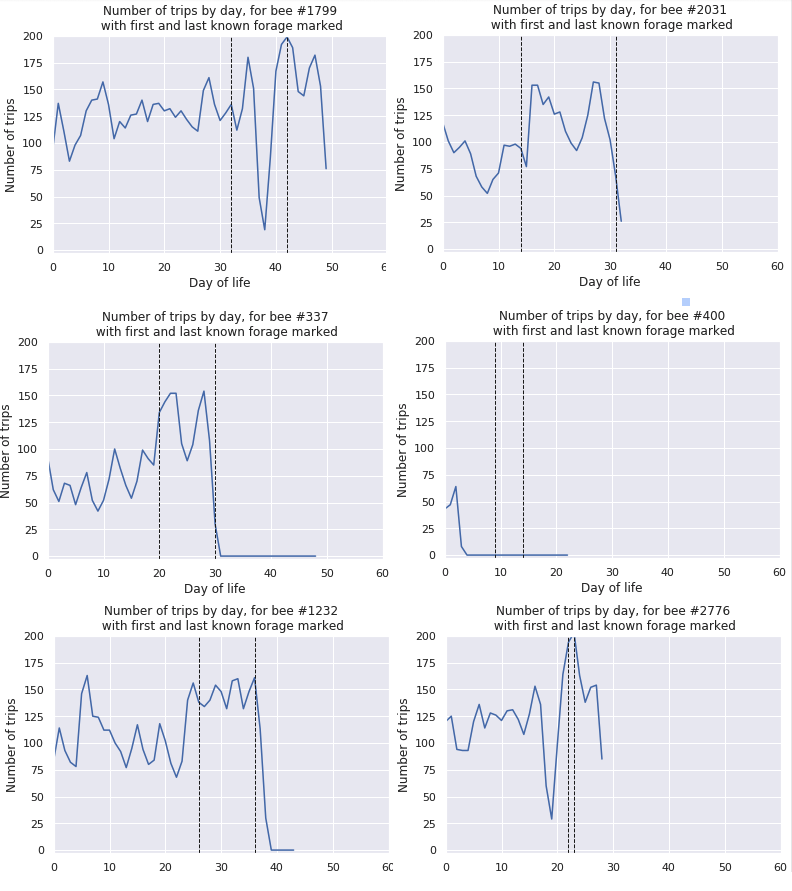
\includegraphics[width=1.0\textwidth]{End-sections/Appendix1/forager-trips.png}
% \caption[beedays-schlegel]{}
\label{fig:beedays-schlegel}
\end{figure}